
\documentclass[journal]{IEEEtran}

\ifCLASSINFOpdf
   \usepackage[pdftex]{graphicx}
  % declare the path(s) where your graphic files are
  % \graphicspath{{../pdf/}{../jpeg/}}
  % and their extensions so you won't have to specify these with
  % every instance of \includegraphics
   \DeclareGraphicsExtensions{.pdf,.jpeg,.png}
\else
  % or other class option (dvipsone, dvipdf, if not using dvips). graphicx
  % will default to the driver specified in the system graphics.cfg if no
  % driver is specified.
  % \usepackage[dvips]{graphicx}
  % declare the path(s) where your graphic files are
  % \graphicspath{{../eps/}}
  % and their extensions so you won't have to specify these with
  % every instance of \includegraphics
  % \DeclareGraphicsExtensions{.eps}
\fi

% correct bad hyphenation here
\hyphenation{op-tical net-works semi-conduc-tor}


\begin{document}

\title{Bare Demo of IEEEtran.cls\\ for IEEE Journals}


\author{Michael~Shell,~\IEEEmembership{Member,~IEEE,}
        John~Doe,~\IEEEmembership{Fellow,~OSA,}
        and~Jane~Doe,~\IEEEmembership{Life~Fellow,~IEEE}% <-this % stops a space
\thanks{M. Shell was with the Department
of Electrical and Computer Engineering, Georgia Institute of Technology, Atlanta,
GA, 30332 USA e-mail: (see http://www.michaelshell.org/contact.html).}% <-this % stops a space
\thanks{J. Doe and J. Doe are with Anonymous University.}% <-this % stops a space
\thanks{Manuscript received April 19, 2005; revised August 26, 2015.}}

% The paper headers
\markboth{Journal of \LaTeX\ Class Files,~Vol.~14, No.~8, August~2015}%
{Shell \MakeLowercase{\textit{et al.}}: Bare Demo of IEEEtran.cls for IEEE Journals}

\maketitle

\begin{abstract}
The abstract goes here.
\end{abstract}

% Note that keywords are not normally used for peerreview papers.
\begin{IEEEkeywords}
IEEE, IEEEtran, journal, \LaTeX, paper, template.
\end{IEEEkeywords}

\IEEEpeerreviewmaketitle



\section{Introduction}

\IEEEPARstart{T}{his} letter presents a deep convolutional
approach for recovering high frequency components in
post-inversion acoustic impedance models. The inversion of
seismic data to obtain acoustic impedance is a frequently
used technique because it offers several advantages: (1) it
facilitates integrated interpretation, (2) stochastic
inversion can improve data's vertical resolution, allowing
sub-seismic features to be more precisely mapped, and (3)
it optimizes the correlation between seismic and petrophysical
properties of the reservoir. Using the seismic data in
deep-water reservoir modeling leads to errors in estimating
the reservoir properties because such data do not allow the
wider understanding of the field under study \cite{Sergio2016}.

Results from a typical post-stack or pre-stack seismic
inversion are band-limited primarily due to missing low
and high frequencies in the wavelet. Consequently, thin beds
are generally poorly resolved \cite{Zhang2012}. The limited
vertical resolution in the conventional seismic data is because 
the frequency of the data is limited in both the low frequencies
and the high frequencies. The inversion process can add low
frequencies to the seismic spectrum through constraint model.
The seismic vertical resolution is the minimal thickness that
can be resolved by seismic. The most accepted value is a quarter
of the wave length (that means that only layers thicker than
that will be detected by seismic acquisition). In larger depths
that value can be as high as 20 meters, which may represent a
significant amount of oil volume being under or overestimated or
mitigate connectivity problems.

In deterministic inversion approaches, the vertical resolution
remains constrained by the seismic bandwidth \cite{Sancevero2005}.
Deterministic inversion is mainly useful for deriving general
trends and highlighting large features in an exploratory stage.
On the other hand, stochastic investion uses random variation
of parameters to reach results with vertical resolution that is
superior to the conventional data. When working with multiple
realizations, selecting the model that best characterizes the
reservoir is difficult, since all of them are equally probable.
Uniqueness problems are an issue mainly addressed by calculating
the mean of different realizations. However, it has been proved
that the mean solution is closer to a bandwidth limited solution,
in such a way that the high frequencies characteristics are lost
\cite{Cook2010}. Another approach to deal with the high frequency
impedance information outside the frequency band of seismic signal
is assuming a blocked model for the earth's impedance \cite{Cook2010}.
This assumption is not always valid, and in some cases the high
frequencies in the inverted impedance are ignored \cite{YuanWang2015}.
Very recent methods aim to enhance the seismic resolution and, by
consequence, achieving an improvement in seismic inversion and
reservoir characterization. \cite{ChenWang2018} use wavelet
frequency-dependent scaling to extends the amplitude spectrum of
high- and low-frequency axes in time domain.

In this letter, we propose a new multichannel and multilayer
Convolutional Neural Network (CNN) model to perform deblurring
in post-inversion acoustic impedance. Each network layer maps
higher level features originating in the previews layers through
one-dimensional convolutional blur kernels. To perform this
mapping, the kernels (also named weights) are adjusted by
minimizing a loss function. The model enhances the resolution
of acoustic impedance images trace by trace, resulting in sharp
images with increased high-frequency band-width and lower noise.
In order to train the model, we perform Maximum-a-Posteriori (MAP)
inversion to obtain a band-limited acoustic impedance model.
Then, the pairs of blur and latent images are normalized and 
presented to the network as input and target, respectively.
The core concept of our architecture is the combination of the
convolutional layers with regression layers, thus the convolutional
layers learn the spatial structures existing in different acoustic
impedance images, while the regression layer proceed the prediction
of the property values. Thus, deblurring the acoustic impedance
models, as a post-inversion refinement process, should lead to a
more accurate interpretation of the impedance models.

The contributions of this work are threefold. First, according
to our knowledge, it is the first to approach inversion resolution 
enhancement through a post-inversion refinement. Second, the proposed deep
learning model effectively recovers the high frequency spectrum absent
in the post-inversion acoustic impedance, yet correcting deformations existing
in thin bodies caused by the inversion process. Third, it contributes
......

The remainder of this letter is organized as follows. Section II
reviews the CNN, a popularly used deep-learning technique.
Section III describes the proposed deblurring approach.
Section \ref{Theoretics} reports the experiments and results, and Section \ref{Conclusion}
concludes our work.
% needed in second column of first page if using \IEEEpubid
%\IEEEpubidadjcol

\section{Theoretical Foundations and Related Works}\label{Theoretics}

Deblurring is generally modeled as the convolution of a blur kernel $k$
with a latent image $I$: 
\begin{equation}
 y = k \otimes I + n
 \label{eq:deblurr}
\end{equation}
where $n$ is the noise. Since $k$, $I$ and $n$ are unknown, the problem 
is highly ill-posed and admits infinite solutions for $k$ and $I$.
Blind deconvolution refers to the inference of the sharp image $I$,
given only the blurry image $y$, without any knowledge regarding the
kernel $k$ and the noise $n$ \cite{Zhang2013}. In contrary, if $k$
is assumed to be known, the approach is called non-blind deconvolution
\cite{Wang2009}.
%Several works have developed different deblurring methods
%for specific purposes. For the last six years, considerable effort has
%been made in single image \cite{Babacan2012,Krishnan2015,Levin2011,Zhang2011}
%and multi-image \cite{sroubek2012,Zhu2012} blind deconvolutions.
Applying blind deconvolution generally implies in making assumptions
on blur kernels and/or on latent images. For example, assuming sparsity
of blur kernel or that natural images have super-Gaussian statistics.
The second assumption leads to the use of image priors on inference process
and, consequently, to the maximum \textit{a posteriori} (MAP) estimation
\cite{Babacan2012}. However, \cite{Levin} show that deblurring methods based
on this prior tend to favor blurry images over original latent images.

The Bayesian inference approach \cite{Levin} outperforms the MAP based
methods. It marginalizes the image from the optimization step, while
estimating the unknown blur. 
%The authors show that it is possible to
%define a class of prior images based on natural image statistics,
%suitable enough to represent sharp images features. This prior
%formulation makes possible to use Bayesian inference in the
%estimation of the unknown image and the blur kernel.
According to \cite{Hacohen13}, defining a gradient prior, by itself,
is not sufficient to reach a sharp image, instead, they search in a data
set for a prior that densely correspond to the blurry image similar
to a sharp image. Even though \cite{Pan2014} suggest a generalization
for the method proposed by \cite{Hacohen13}, it still requires a similar
reference image, which is not always available.

%It has been demonstrated that 
The methods described previously fail when applied to real world
blurry images \cite{Lai2016} and take a severe computational cost
\cite{Chakrabarti2016}. In contrast, the learning-based methods
have gained attention with the resumption and recent advances in
convolutional neural networks (CNN). The adequate hyper-parameter
adjustment allows CNN to learn non-linear function or blur kernels.
Thus, deblurring becomes a function of a blurry image $I$ and a set
of parameters $p$ as \ref{eq:deblur}
\begin{equation}
 y = \sigma(I,p)
 \label{eq:deblur}
\end{equation}
Learning-based methods focus on developing a model to learn the function
$\sigma$ and to perform non-blind deblurring \cite{Chakrabarti2016}.
\cite{Sun2015} teaches a CNN to recognize motion kernels and performs non-blind
deconvolution in dense motion field estimate, in addition, \cite{Hradis2015}
minimize regularized $l_2$ in order to perform text deblurring.

\section{Data and Methods}\label{Method}
%The workflow of the proposed method consists of the following
%steps:
%\begin{itemize}
% \item Obtaining blurry images through MAP acoustic inversion;
% \item Train the convolutional model with the pair of high and low resolution images;
% \item Test the model with different blurry images;
% \item Assess the result for the testing output.
%\end{itemize}

\subsection{Data Set}
To evaluate the proposed deblurring method, an acoustic
impedance data set is collected. \footnote{Available at https://github.com/SCRFpublic/Stanford-VI-E/tree/master/Acoustic\%20Impedance} %Badbox aqui
The data set contains a cube of acoustic impedance values from the updated Stanford VI reservoir \cite{Lee2012}, which is represented by a three-dimensional regular stratigraphic model. The cube contains 150x200x200 cells and the dimensions of each cell are $25$ meters horizontally and $1$ meter vertically. The model represents a fluvial channel system composed of three layers: the lowest one represents deltaic deposits (layer 3), the middle layer represents meandering channels (layer 2) and the first layer sinuous channels, deposited in the fluvial channel system. \footnote{See \cite{Castro2005} for more details about methodologies and model parameters.} Some sample images from Stanford VI are shown in Fig. \ref{fig_examples}
\begin{figure}[!t]
\centering
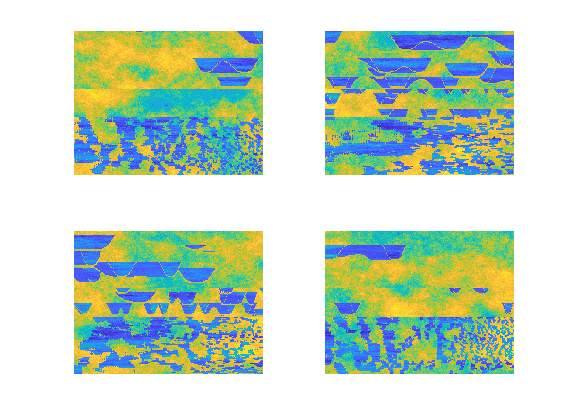
\includegraphics[width=2.5in]{Figs/Examples}
\DeclareGraphicsExtensions.
\caption{Examples.}
\label{fig_examples}
\end{figure}
Even though the data has been synthetically generated through flux
simulation, the layers represent geological bodies of high importance
in reservoir characterization, such as channels connections and theirs
discontinuity...

In a realistic scenario, the number of hard data available for
training and validating supervised models is scarce. In order
to address this common issue, we performed experiments
restricting the amount of training data set to 50\%, 30\% and
10\% of the available data. The results using 50\% and 30\% did
not show significant difference in the frequency spectrum,
whereas 10\% showed more significant discrepancies in the
amplitude recovering and additional noise in higher frequencies
(Fig. \ref{fig_imgs}). Therefore, for the following experiments
we adopted 30\% of available data as training data set, once we
observed it as the minimum amount of data to keep the model learning
capability.
\begin{figure}[!t]
\centering
\includegraphics[width=2.5in]{Figs/images}
\DeclareGraphicsExtensions.
\caption{Examples.}
\label{fig_imgs}
\end{figure}

To build the training data set we carry out the \textit{Maximum-a-Posteriori} (MAP) \cite{Buland2003,Figueiredo2012} inversion using the high resolution acoustic
impedance. In order to proceed the inversion, we created a Ricker wavelet with
frequency band-width from $0Hz$ to $60Hz$, with which the synthetic seismic was
calculated through the forward model. Additionally, a low frequency
model is calculated by applying a low-pass filter with $4Hz$ cutting frequency.
Thus, the inverted acoustic impedance cube is calculated and the pair of truth
and inverted images compose the training data set. As expected, the inverted
acoustic impedance band-width is restricted to the wavelet band-width with
addition of the frequencies existing in the low frequency model. Due to the 1D
convolution adopted in this work, the available data set contains $30000$ trace
samples with $200$ cell along the depth.

\subsection{Proposed Architecture}

We propose a four-layer multichannel CNN architecture for deblurring
post-inversion acoustic impedance images and recovering high
frequency of thin layers. The model takes in each input channel the
trace of the blurred acoustic impedance and the respective seismic
data. By doing so, the network is able to learn with the acoustic
impedance data associated with the local high frequency seismic.
The model consists of one convolutional layer and one locally connected
layer, each one of them followed by max pooling. The output of the
locally connected is flatted and two fully connected layers are
added in the end (Fig. ).

The first convolutional layer deblurs the lower features in
the input traces. Following, higher features are deblurred
and individualized through a locally-connected layer \cite{},
which performs a one-dimensional convolution
with unshared weights. Thus, instead of performing standard
convolution, the weights of the learned kernel matrices are not
shared across the input. %This technique allowed learning 
%individual features in each trace example presented to the network.
The number of filters in the convolutional and locally connected
layers is 50 and 100, respectively. As long as the number of
filters increases from the first to the second layer, the size
of each filter decreases from 20 to 10. This way, we note that
the network learns thinner geological bodies in the second layer.

We used rectified linear unit (ReLU) function that is one
of the most popular and efficient activation functions for
CNNs. There are advantages of using ReLU such as efficient
computation, and gradient propagation. The network uses
Adam to optimize the loss function. This algorithm
combines the AdaGrad and RMSProp methods and converges more efficiently in
comparison to gradient descent, stochastic gradient descent, AdaGrad
and RMSProp \cite{Kingma2014}. The Mean Absolute Error (MAE) is the
loss function minimized in the training process. Additionally, we use
a batch size of 10 traces.

\section{Experiment and Discussion}\label{Experiments}
Here, we validate the proposed post-inversion deblurring method.
The parameters settings for the model training are presented.
Next, the experimental results are given for the proposed method,
as well as the comparison methods.

\subsection{Model Training}
In order to train the CNN model, $80\%$ of the acoustic impedance images
is used to infer the blur filters and $20\%$ of the images is used as 
validation samples. Due to the predefined hyperbolic tangent
sigmoid (\textit{tansig}) transfer function in the last layer, we
normalized the acoustic impedance to values between 0 and 1,
and the results are presented in terms of this normalization.

\subsection{Deblurring Post-Inversion Acoustic Impedance}

The results show a frequency spectrum very similar to the raw data.
The deblurred images show a good recovery of high frequency events
(thin layers), which are better noticed in the intersections between
two channels (Fig. \ref{ImSec26}).
\begin{figure}[!t]
\centering
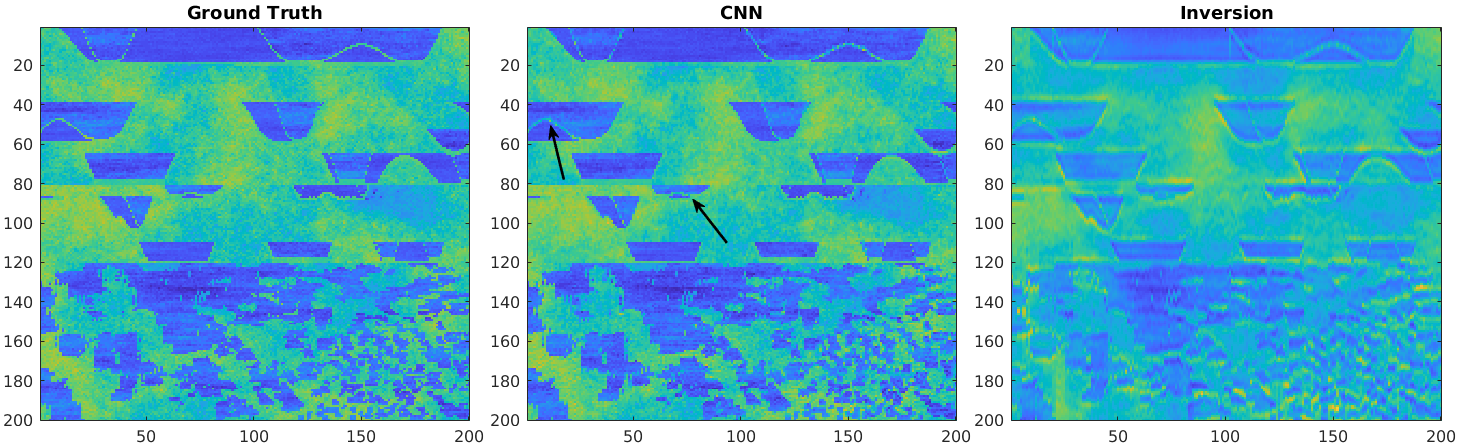
\includegraphics[width=2.5in]{Figs/ImSec26}
\DeclareGraphicsExtensions.
\caption{Examples.}
\label{ImSec26}
\end{figure}
It should be pointed out that the horizontal resolution seem to be better enhanced when compared to the vertical resolution, which can be an effect of the wavelet signature and/or the deconvolution process. The increase in the horizontal resolution is particularly important, since that's the situation where the layers get thinner and the porosity decreases, thus decreases the impedance contrast and, therefore, its seismic response. The vertical resolution improvement is essential to evaluate the vertical connectivity in the reservoir (thin layers of shale may act as barriers for the water injection and affect the production and pressurization of the reservoir). Besides significant improvements in the resolution, the model managed to correct some geometric deformations created during the inversion process (Fig. \ref{ImSec36}), which usually occurs in smaller depositional features (smaller channels).
\begin{figure}[!t]
\centering
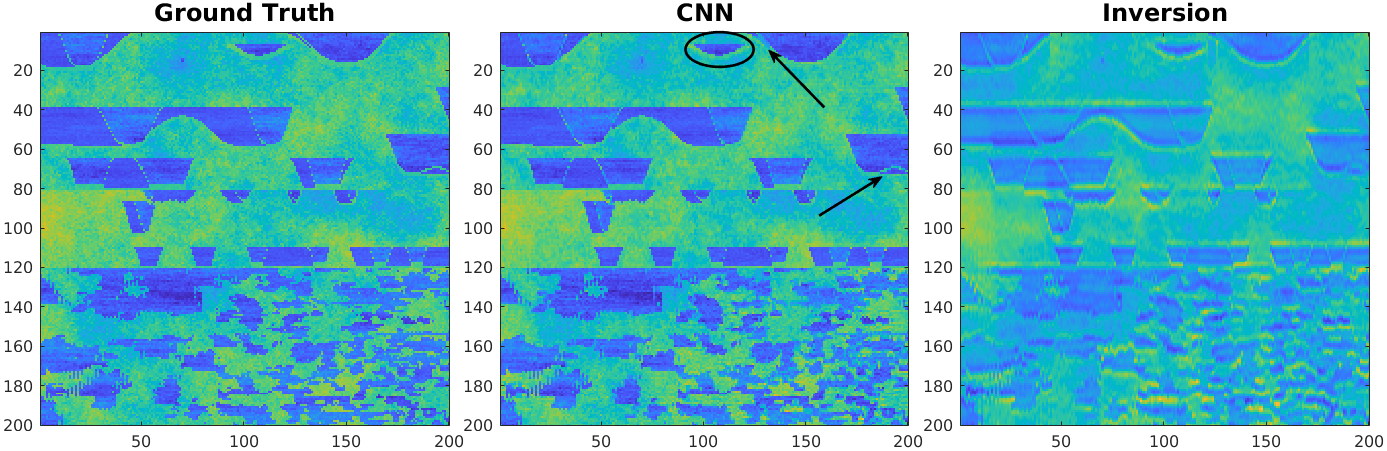
\includegraphics[width=2.5in]{Figs/ImSec36}
\DeclareGraphicsExtensions.
\caption{Examples.}
\label{ImSec36}
\end{figure}

\begin{table}[!t]
\renewcommand{\arraystretch}{1.3}
\caption{Table of metric values for wedges with acoustic impedance normalized to $0$ and $1$.}
\label{table_caso_1}
\centering
\begin{tabular}{|c||c||c|}
\hline
 \textbf{Image Section} & \textbf{\textit{Wiener Filter (dB)}} & \textbf{\textit{Our (dB)}}\\
\hline
Inline Section & $0.1$ & $0.1$ \\
\hline
Crossline Section & $0.1$ & $0.1$ \\
\hline
\end{tabular}
\end{table}

\section{Conclusion} \label{Conclusion}
In summary, we showed that the CNN has  Moreover, we introduced a simple architecture that combines convolutional, regression and locally connected layers. We demonstrated that the CNN achieved reasonable results regarding the high frequency recovering in seismic inversion data. The methodology is promising for deblurring post-inversion acoustic impedance due to its capability to learn one-dimensional blur kernels and recovering two-dimensional geometric features (such as deposition borders and thin layers). One suggestion for the workflow input data is using the shallower portion of the seismic, since most geological features tend to repeat themselves (fractal) where the frequency spectrum is broader in the high frequencies (the frequency amplitude decreases exponentially with depth, due to attenuation and dispersion effects during propagation). This way we could get a more realistic and comprehensive training data.

\section*{Acknowledgment}

The authors would like to thank Conselho Nacional de Pesquisa e Desenvolvimento, Fundação de Amparo à Pesquisa e Inovação do Estado de Santa Catarina and Petrobras for their support and availability during the work.

\ifCLASSOPTIONcaptionsoff
  \newpage
\fi

\begin{thebibliography}{1}
\bibitem{Sergio2016}
S. S. Sancevero, A. Z. Remacre, R. S. Portugal, "O papel da inversão para a impedância no processo de caracterização sísmica de reservatórios." in Revista Brasileira de Geofísica, p. 495-512, v. 24, 2006.

\bibitem{xiaoiu}
X. Xiaoyu, L. Yun, S. Desheng, G. Xiangyu, and W. Huifeng, "Studying the effect of expanding low or high frequency on post-stack seismic inversion," in SEG Technical Program Expanded Abstracts 2012, pp. 1-5, September 2012.

\bibitem{Zhang2012}
R. Zhang and M. K. Sen and S. Phan and S. Srinivasan, "Stochastic and deterministic seismic inversion methods for thin-bed resolution", Journal of Geophysics and Engineering, V. 9, N. 5, 2012.

\bibitem{Sancevero2005}
S. S. Sancevero and A. Z. Remacre and R. de S. Portugal and E. C. Mundim, "Comparing deterministic and stochastic seismic inversion for thin-bed reservoir characterization in a turbidite synthetic reference model of Campos Basin, Brazil", The Leading Edge, v. 24, num. 11, pp. 1168-1172, 2005. 

\bibitem{Cook2010}
D. Cooke and J. Cant and A. Santos and  P. Wa, Australia,  "Model-based Seismic Inversion: Comparing deterministic and Probabilistic approaches". CSEG Recorder, 2010. 

\bibitem{YuanWang2015}
S. Yuan and S. Wang and C. Luo and Y. He, "Simultaneous multitrace impedance inversion with transform-domain sparsity promotion", Geophysics, pp. 71-80, v. 80, n. 2, 2015.

\bibitem{ChenWang2018}
S. Chen and Y. Wang, "Seismic Resolution Enhancement by Frequency-Dependent Wavelet Scaling," in IEEE Geoscience and Remote Sensing Letters, vol. PP, no. 99, pp. 1-5.

%\bibitem{Krizhevsky2012}
%A. Krizhevsky, I. Sutskever, G. E. Hinton, "Imagenet classification with deep convolutional neural networks: Advances in neural information processing systems," , pp. 1097–1105, 2012.

%\bibitem{AbdelHamid2014}
%O. Abdel-Hamid, A.-r. Mohamed, H. Jiang, L. Deng, G. Penn, and D. Yu, "Convolutional neural networks for speech recognition," in IEEE/ACM Transactions on audio, speech, and language processing, num. 22, pp. 1533–1545, 2014.

%\bibitem{Farfade2015}
%S. S. Farfade, M. J. Saberian, and L.-J. Li, 2015, "Multi-view face detection using deep convolutional neural networks," in Proceedings of the 5th ACM on International Conference on Multimedia Retrieval, ACM, pp. 643–650.

%\bibitem{S_Ji2013}
%S. Ji,W. Xu, M. Yang, K. Yu, 2013, "3d convolutional neural networks for human action recognition," in IEEE transactions on pattern analysis and machine intelligence, num. 35, p. 221–231.

%\bibitem{Qian}
%Q. Feng, Y. Miao, S. Ming-Jun, W. Yaojun, H. Guangmin, "Seismic facies recognition based on prestack data using deep convolutional autoencoder,".

%\bibitem{Liu2017}
%L. Lihui, L. Rong, L. Jianhai, Y. Wenkui, "Seismic Lithofacies Computation Method Based on Deep Learning," in International Geophysical Conference, pp. 649-652, April 2017.

\bibitem{Zhang2013}		H. Zhang, D. Wipf and Y. Zhang, "Multi-image Blind Deblurring Using a Coupled Adaptive Sparse Prior," 2013 IEEE Conference on Computer Vision and Pattern Recognition, Portland, OR, 2013, pp. 1051-1058.

\bibitem{Babacan2012}		S. D. Babacan, R. Molina, M. N. Do, and A. K. Katsaggelos, ``Bayesian blind deconvolution with general sparse image priors.'' in Proceedings of European Conference on Computer Vision (ECCV), pp. 341–355, 2012.
%\bibitem{Krishnan2015}		D. Krishnan, T. Tay, and R. Fergus, ``Blind deconvolution using anormalized sparsity measure.'' In CVPR, 2011.
%\bibitem{Levin2011}		A. Levin, Y. Weiss, F. Durand, and W. T. Freeman. ``Efficient marginal likelihood optimization in blind deconvolution.'' In CVPR, 2011.
\bibitem{Wang2009}		C. Wang, L. Sun, Z. Chen, S. Yang and J. Zhang, "High-quality non-blind motion deblurring," 2009 16th IEEE International Conference on Image Processing (ICIP), Cairo, 2009, pp. 153-156.
%\bibitem{Zhang2011}		H. Zhang, J. Yang, Y. Zhang, N. M. Nasrabadi, and T. S. Huang, ``Close the loop: Joint blind image restoration and recognition with sparse representation prior.'' in ICCV, 2011. 
%\bibitem{sroubek2012}		F. Šroubek and P. Milanfar, ``Robust multichannel blind deconvolution via fast alternating minimization.'' in IEEE Trans. on Image Processing, pp. 1687–1700, 2012.
%\bibitem{Zhu2012}		X. Zhu, F. Šroubek, P. Milanfar, ``Deconvolving PSFs for a better motion deblurring using multiple images.'' in ECCV, 2012.
\bibitem{Levin}			A. Levin, Y. Weiss, F. Durand, and W. T. Freeman. ``Understanding and evaluating blind deconvolution algorithms.'' In IEEE Proceedings of International Conference on Computer Vision and Pattern Recognition (CVPR), pp. 1964–1971.
\bibitem{Hacohen13}		Y. Hacohen, E. Shechtman, and D. Lischinski, ``Deblurring by example using dense correspondence.'' In IEEE Proceedings of International Conference on Computer Vision (ICCV), pp. 2384–2391, 2013.
\bibitem{Pan2014}		J. Pan, Z. Hu, Z. Su, and M. H. Yang, ``Deblurring face images with exemplars.'' In Proceedings of European Conference on Computer Vision (ECCV), pp. 47–62. Springer, 2014.
\bibitem{Lai2016}		W.S. Lai, J. B. Huang, Z. Hu, N. Ahuja, and M. H. Yang, ``A comparative study for single image blind deblurring.'' In IEEE Proceedings of International Conference on Computer Vision and Pattern Recognition (CVPR). IEEE, 2016.
\bibitem{Chakrabarti2016}	A. Chakrabarti, ``A neural approach to blind motion deblurring.'' In Proceedings of European Conference on Computer Vision (ECCV), pp. 221–235. Springer, 2016.
\bibitem{Sun2015}		J. Sun, W. Cao, Z. Xu, and J. Ponce, ``Learning a convolutional neural network for non-uniform motion blur removal.'' In IEEE Proceedings of International Conference on Computer Vision and Pattern Recognition (CVPR), pp. 769–777, 2015.
\bibitem{Hradis2015}		M. Hradiš, J. Kotera, P. Zemcı́k, and F. Šroubek, ``Convolutional neural networks for direct text deblurring.'' In Proceedings of British Machine Vision Conference (BMVC), 2015.

\bibitem{Kingma2014}
D. P. Kingma and J. Ba. “Adam: A method for stochastic optimization.” Unpublished paper, 2014. [Online]. Available: https://arxiv.org/abs/1412.6980

\bibitem{Lee2012}
Lee, J. and Mukerji, T., 2012, "The Stanford VI-E reservoir: A synthetic data set for joint seismic-EM time-lapse monitoring algorithms": 25th Annual Report, Stanford Center for Reservoir Forecasting, Stanford University, Stanford, CA.

\bibitem{Castro2005}
Castro, S., Caers, J., and Mukerji, T., 2005, “The Stanford VI reservoir”: 18th Annual Report, Stanford Center for Reservoir Forecasting, Stanford University, Stanford, CA.

\bibitem{Buland2003}
A. Buland,  and H. Omre, ``Bayesian linearized avo inversion,'' In Geophysics, 2003, pp. 185--198.

\bibitem{Figueiredo2012}
L. P. Figueiredo, M. Santos, M. Roisenberg, G. Neto, and W. Figueiredo, ``Bayesian framework to wavelet estimation and linearized acoustic inversion,'' in Geoscience and Remote Sensing Letters, pp. 1--5, 2012.

\end{thebibliography}

%\begin{IEEEbiography}{Michael Shell}
%Biography text here.
%\end{IEEEbiography}

% if you will not have a photo at all:
%\begin{IEEEbiographynophoto}{John Doe}
%Biography text here.
%\end{IEEEbiographynophoto}


%\begin{IEEEbiographynophoto}{Jane Doe}
%Biography text here.
%\end{IEEEbiographynophoto}

\end{document}


\grid
\grid
